% --------------------------------------------------------------
% This is all preamble stuff that you don't have to worry about.
% Head down to where it says "Start here"
% --------------------------------------------------------------
 
\documentclass[12pt]{article}

\usepackage[margin=1in]{geometry} 
\usepackage{amsmath,amsthm,amssymb,listings,xcolor,graphicx,enumerate,framed}
 
\newenvironment{solution}{\begin{proof}[Solution]}{\end{proof}}

\definecolor{codegreen}{rgb}{0,0.6,0}
\definecolor{codegray}{rgb}{0.5,0.5,0.5}
\definecolor{codepurple}{rgb}{0.58,0,0.82}
\definecolor{backcolour}{rgb}{0.97,0.97,0.97}
\lstdefinestyle{pystyle}{
    backgroundcolor=\color{backcolour},   
    commentstyle=\color{codegreen},
    keywordstyle=\color{magenta},
    numberstyle=\tiny\color{codegray},
    stringstyle=\color{codepurple},
    basicstyle=\ttfamily\small,
    breakatwhitespace=false,         
    breaklines=true,                 
    captionpos=b,                    
    keepspaces=true,                 
    numbers=left,                    
    numbersep=5pt,                  
    showspaces=false,                
    showstringspaces=false,
    showtabs=false,                  
    tabsize=2
}
\lstset{style=pystyle}

\graphicspath{{./figures}}
 
\begin{document}
 
\title{Homework 2: Vectors, Subspaces, and Norms}
\author{Matthew Luyten\\ %replace with your name
ECE6250}

\maketitle

\begin{enumerate}
\item[Problem 2.1] Summary and Context of Vectors/Subspaces/Norms

This week we covered vectors, subspaces, and norms. These are fundamental concepts in linear algebra,
and therefore, they are foundational concepts in DSP. Vector spaces make up a framework for how we
work in linear algebra, so it is very important that we define rules and develop an understanding
of them. We also talked about norms, which are a measurement of distance. I've studied these in an
undergraduate data science course where we used these norms to determine the distance between points
in order to cluster them. Understanding the norms, how they work, and what they say about two points
is very important in data science and scientific modeling. Using different norms can yield very
different clustrering results.

This week's lectures laid the groundwork to introduce hilbert spaces, which are a very powerful tool
that allow us to estimate signals using other functions, much like the fourier transform. However, to use
this tool, one must understand vector spaces and bases.

\newpage

\item[Problem 2.2] Consider vector $V=\{\bold{v_1},\bold{v_2}, \bold{v_3}, \bold{v_4}\}$ in $\mathbb{R}^{2\times2}$, prove 1, 2, 3, and 4.

\[
\bold{v_1}=
\begin{bmatrix}
    1 & 0\\
    0 & 0
\end{bmatrix}
, \bold{v_2}=
\begin{bmatrix}
    0 & 1\\
    0 & 0
\end{bmatrix}
, \bold{v_3}=
\begin{bmatrix}
    0 & 0\\
    1 & 0
\end{bmatrix}
, \bold{v_4}=
\begin{bmatrix}
    0 & 0\\
    0 & 1
\end{bmatrix}
\]

\noindent
1. The span of $V=\mathbb{R}^{2\times2}$

\begin{enumerate}[\noindent]
\item Vector $\bold{x}=\begin{bmatrix}a_1&a_2\\a_3&a_4\end{bmatrix}$ can be expressed
as a linear combination of $V$

$\bold{x}=a_1 \bold{v_1}+a_2 \bold{v_2}+a_3\bold{v_3}+a_4\bold{v_4}$

$\bold{x}=\begin{bmatrix}a_1&a_2\\a_3&a_4\end{bmatrix}$ can represent every vector in 
$\mathbb{R}^{2\times2}$

\begin{framed}
$\therefore V$ spans $\mathbb{R}^{2\times2}$
\end{framed}

\end{enumerate}

2. $V$ is linearly independent in $\mathbb{R}^{2\times2}$

$V$ is linearly independent if $\sum_{n=1}^{4}a_n \bold{v_n} = \bold{0}$ only when 
$A = \{a_1,a_2,a_3,a_4\} = \bold{0}$

$\bold{x}=a_1 \bold{v_1}+a_2 \bold{v_2}+a_3\bold{v_3}+a_4\bold{v_4}$
$\bold{x}=\begin{bmatrix}a_1&a_2\\a_3&a_4\end{bmatrix}$ can only equal $\bold{0}$ when $A=\bold{0}$

\begin{framed}
$\therefore V$ is linearly independent in $\mathbb{R}^{2\times2}$
\end{framed}

3. $V$ is a basis for $\mathbb{R}^{2\times2}$ 

$V$ spans $\mathbb{R}^{2\times2}$ (see 1) and $V$ is linearly independent in $\mathbb{R}^{2\times2}$ (see 2)

\begin{framed}
$\therefore$ $V$ is a basis for $\mathbb{R}^{2\times2}$ 
\end{framed}

\pagebreak

\item[Problem 2.3] Let $C=[-1,1]$, $C_e=\{ f\in C: f$ is even\}, $C_o=\{ f\in C: f$ is out\}

a) Prove that $C_o$ and $C_e$ are both subspaces of $C$

$C_o$ closed under vector addition in $C$? Let $f(x),g(x)\in C_o$

\[h(x)=f(x)+g(x)\]
\[h(-x)=f(-x)+g(-x)\]
\[h(-x)=-f(x)-g(x)\]
\[h(-x)=-h(x)\]
\[h(x)\in C_o\]
\[\therefore C_o\text{ is closed over vector addition}\]

$C_o$ closed under scalar multiplication in $C$? Let $f(x)\in C_o$, $a\in \mathbb{R}$

\[h(x)=a f(x)\]
\[h(-x)=af(-x)\]
\[h(-x)=-af(x)\]
\[h(-x)=-h(x)\]
\[h(x)\in C_o\]
\[\therefore C_o\text{ is closed over scalar multiplication}\]

$C_o$ contains the zero vector in $C$? Let $f(x)\in C_e$

\[z(x)=0\]
\[f(x) + z(x) = f(x) + 0 = f(x)\]
\[z(x)\text{ is the zero vector}\]
\[z(-x) = 0\]
\[-z(x) = 0\]
\[z(-x) = -z(x)\]
\[\therefore C_o\text{ contains the zero vector}\]

\begin{framed}
$C_o$ contains the zero vector and is closed under vector addition and scalar multiplication, so
$C_o$ is a subspace of $C$
\end{framed}

$C_e$ closed under vector addition in $C$? Let $f(x),g(x)\in C_o$

\[h(x)=f(x)+g(x)\]
\[h(-x)=f(-x)+g(-x)\]
\[h(-x)=f(x)+g(x)\]
\[h(-x)=h(x)\]
\[h(x)\in C_e\]
\[\therefore C_e\text{ is closed over vector addition}\]

$C_e$ closed under scalar multiplication in $C$? Let $f(x)\in C_e$, $a\in \mathbb{R}$

\[h(x)=a f(x)\]
\[h(-x)=af(-x)\]
\[h(-x)=af(x)\]
\[h(-x)=h(x)\]
\[h(x)\in C_e\]
\[\therefore C_e\text{ is closed over scalar multiplication}\]

$C_e$ contains the zero vector? Let $f(x)\in C_e$

\[z(x)=0\]
\[f(x) + z(x) = f(x) + 0 = f(x)\]
\[z(x)\text{ is the zero vector}\]
\[z(-x) = 0\]
\[z(x) = 0\]
\[z(-x) = z(x)\]
\[\therefore C_e\text{ contains the zero vector}\]

\begin{framed}
$C_e$ contains the zero vector and is closed under vector addition and scalar multiplication, so
$C_e$ is a subspace of $C$
\end{framed}

b) Prove that $C_o$ and $C_e$ are orthogonal subspaces

\[\langle x,y\rangle=\int_{-1}^1f(x)g(x)dx\]
\[\int_{-1}^1f(x)g(x)dx=\int_{-1}^0f(x)g(x)dx+\int_0^1f(x)g(x)dx\]
\[f(-x)=f(x),\quad g(-x)=g(x)\]
\[\int_{-1}^0f(x)g(x)dx=-\int_0^1f(x)g(x)dx\]
\[\int_{-1}^1f(x)g(x)dx=\int_0^1f(x)g(x)dx-\int_0^1f(x)g(x)dx=0\]

\begin{framed}
$\langle x,y\rangle=0\therefore C_o$ and $C_e$ are orthogonal subspaces
\end{framed}

\newpage

\item[Problem 2.4] Let $V$ is all real number numbers greater than 0

a) Is $V$ under $\boxplus$ and $\boxdot$ a vector space? Let
$x\boxplus y=xy+1$ for all $x,y\in V$, and $a\boxdot x=a^2x$ for all $x,y\in V$

\[x\boxplus y=xy+1\]
\[y\boxplus x=yx+1\]
\[x\boxplus y=y\boxplus x\quad\text{ (Commutative Satisfied)}\]

\[x\boxplus (y\boxplus z)=xyz+x+1\]
\[(x\boxplus y)\boxplus z=xyz+z+1\]
\[x\boxplus (y\boxplus z)\neq (x\boxplus y)\boxplus z\quad\text{ (Associative Not Satisfied)}\]

\[x\boxplus z=x\]
\[z=\bold{0} =1+\frac{1}{x}\quad\text{ ($V$ Has No Unique Zero Vector)}\]
\[(\therefore \text{$V$ Has No Vector $-x$ That Satisfies $x\boxplus (-x)=\bold{0}$})\]

\[a\boxdot (x\boxplus y)=a^2xy+a^2\]
\[(a\boxdot x)\boxplus (a\boxdot y)=a^4xy+1\]
\[a\boxdot (x\boxplus y)\neq(a\boxdot x)\boxplus (a\boxdot y)\quad\text{ (Distributive Not Satisfied)}\]

\[(ab)\boxdot x=(ab)2x=a^2b^2x\]
\[a(b\boxdot x)=a^2b^2x\]
\[(ab)\boxdot x=a(b\boxdot x)\quad\text{ (Associative Satisfied)}\]

\[1\boxdot x=1^2x\]
\[1\boxdot x=x\quad\text{ (Multiplicitive Satisfied)}\]

\[0\boxdot x\neq\bold{0},\quad\bold{0}\notin V\quad\text{ (Additive Not Satisfied)}\]

\[a\boxdot x\boxplus b\boxdot y\, \quad x,y\in V\, \quad \forall a,b\in\mathbb{R}\]
\[a\boxdot x\boxplus b\boxdot y=(a^2x)(a^2y)+1=a^4xy+1\]
\[a^4xy+1 \in \mathbb{R}\quad\text{$V$ is closed under vector addition and scalar multiplication}\]

\begin{framed}
$V$ is not a vector space under $\boxplus$ and $\boxdot$.

$V$'s $\boxplus$ opperator does not satisfy the Associative Identity,
has no zero vector $\bold{0}$ that $x+\bold{0}=x\forall x\in S$, and has no vector $-x$ such that 
$x+(-x)=\bold{0}$

$V$'s $\boxdot$ opperator does not satisfy the Distributive and Additive Identities
\end{framed}

b) Is $V$ under $\boxplus$ and $\boxdot$ a vector space? Let
$x\boxplus y=xy$ for all $x,y\in V$, and $a\boxdot x=x^a$ for all $x,y\in V$

\[x\boxplus y=xy\]
\[y\boxplus x=yx\]
\[x\boxplus y=y\boxplus x\quad\text{ (Commutative Satisfied)}\]

\[x\boxplus (y\boxplus z)=x(yz)=xyz\]
\[(x\boxplus y)\boxplus z=(xy)z=xyz\]
\[x\boxplus (y\boxplus z)=(x\boxplus y)\boxplus z\quad\text{ (Associative Satisfied)}\]

\[x\boxplus z=x\]
\[z=1=\bold{0}\quad\text{ ($V$ Has A Unique Zero Vector)}\]

\[-x=\frac{1}{x}\]
\[x\boxplus(-x)=\bold{0}\]
\[x(1/x)=1=\bold{0}\]
\[\text{$V$ Has A Vector $-x$ That Satisfies $x\boxplus (-x)=\bold{0}$}\]

\[a\boxdot (x\boxplus y)=(xy)^a=x^ay^a\]
\[(a\boxdot x)\boxplus (a\boxdot y)=x^ay^a\]
\[a\boxdot (x\boxplus y)=(a\boxdot x)\boxplus (a\boxdot y)\quad\text{ (Distributive Satisfied)}\]

\[(ab)\boxdot x=x^{ab}\]
\[a(b\boxdot x)=(x^b)^a=x^{ab}\]
\[(ab)\boxdot x=a(b\boxdot x)\quad\text{ (Associative Satisfied)}\]

\[1\boxdot x=x^1\]
\[1\boxdot x=x\quad\text{ (Multiplicitive Satisfied)}\]

\[0\boxdot x=x^0=1=\bold{0}\]
\[0\boxdot x=\bold{0},\quad\bold{0}\in V\quad\text{ (Additive Satisfied)}\]

\[a\boxdot x\boxplus b\boxdot y\, \quad x,y\in V\, \quad \forall a,b\in\mathbb{R}\]
\[a\boxdot x\boxplus b\boxdot y=(x^a)(y^b)\]
\[x^ay^b \in V\quad\therefore\text{$V$ is closed under vector addition and scalar multiplication}\]

\begin{framed}
$V$ is a vector space under $\boxplus$ and $\boxdot$.
\end{framed}

\newpage

\item[Problem 2.5] Prove the "reverse triangle inequality" holds in a normed vector space

Start by expanding $\|x-y\|^2$

\[\|x-y\|^2=\langle x-y,x-y\rangle\]
\[\|x-y\|^2=\langle x,x-y\rangle-\langle y,x-y\rangle\]
\[\|x-y\|^2=\langle x,x\rangle-\langle x,y\rangle-\langle y,x\rangle+\langle y,y\rangle\]
\[\|x-y\|^2=\|x\|^2-2\langle x,y\rangle+\|y\|^2\]

Check if "reverse" triangle inequality is true:

\[\|x\|-\|y\|\le \|x-y\|\]
\[(\|x\|-\|y\|)^2\le \|x-y\|^2\]
\[\|x\|^2+\|y\|^2-2\|x\|\:\|y\|\le \|x\|^2+\|y\|^2-2\langle x,y\rangle\]

\begin{framed}
Given the Cauchy-Schwarz Inequality ($|\langle x,y\rangle|\le\|x\|\:\|y\|$): 

$\|x\|-\|y\|\le \|x-y\|$ with equality iff $x$ and $y$ are colinear.
\end{framed}

\newpage

\item[Problem 2.6] Let $\|\dot\|_p$ be the $\ell_p$ norm for vectors in $\mathbb{R}^N$
Given: $(a_1+a_2)^\alpha\ge a_1^\alpha+a_2^\alpha$ for $\alpha\ge1$

a) Prove $\|x\|_p\le\|x\|_1$ for all $x\in\mathbb{R}$, $p\ge 1$

\[\|x\|_p=(\sum_{n=1}^{N}|x_n|^p)^{1/p}\]
\[\|x\|_1=(\sum_{n=1}^{N}|x_n|^1)^1\]
\[(\sum_{n=1}^{N}|x_n|^p)^{1/p}\le(\sum_{n=1}^{N}|x_n|^1)^1\]
\[\sum_{n=1}^{N}|x_n|^p\le(\sum_{n=1}^{N}|x_n|)^p\]
\[(x_1^p+x_2^p+...+x_n^p)\le(x_1+x_2+...+x_n)^p\]

\begin{framed}
$(a_1+a_2)^\alpha\ge a_1^\alpha+a_2^\alpha$ for $\alpha\ge1 \therefore \|x\|_p\le\|x\|_1$\
for all $x\in\mathbb{R}$, $p\ge 1$
\end{framed}

b) Prove that $\|x\|_p\le\|x\|_q$ for all $x\in\mathbb{R}$, $1\le q\le p\le\infty$

\[\text{Let $\beta$ be a real number greater than 1 where $p=\beta q$}\]
\[\|x\|_p=(\sum_{n=1}^{N}|x_n|^{\beta q})^{\frac{1}{\beta q}}\]
\[\|x\|_q=(\sum_{n=1}^{N}|x_n|^q)^\frac{1}{q}\]
\[(\sum_{n=1}^{N}|x_n|^{\beta q})^{\frac{1}{\beta q}}\le(\sum_{n=1}^{N}|x_n|^q)^\frac{1}{q}\]
\[\sum_{n=1}^{N}|x_n|^{\beta q}\le(\sum_{n=1}^{N}|x_n|^q)^\beta\]
\[(x_1^p+x_2^p+...+x_n^p)\le(x_1+x_2+...+x_n)^p\]

\begin{framed}
$(a_1+a_2)^\alpha\ge a_1^\alpha+a_2^\alpha$ for $\alpha\ge1 \therefore \|x\|_p\le\|x\|_n$ 
for all for all $x\in\mathbb{R}$, $1\le q\le p\le\infty$
\end{framed}


\newpage

\item[Problem 2.7] Visualizing $\mathbb{R}^2$ with the unit ball

a) Find $r = \|x\|_p$ for $p=1,2,\infty$ and sketch $x$ and $rB$

\begin{framed}
\[\|x\|_1=3+2=5\]\
\end{framed}

\begin{figure}[h]not a valid norm
\end{figure}

\begin{framed}
\[\|x\|_2=\sqrt{3^2+2^2}=\sqrt{13}\]
\end{framed}
\begin{figure}[h]
    \caption{Plot of $x$ and $rB_2$}
    \centering
    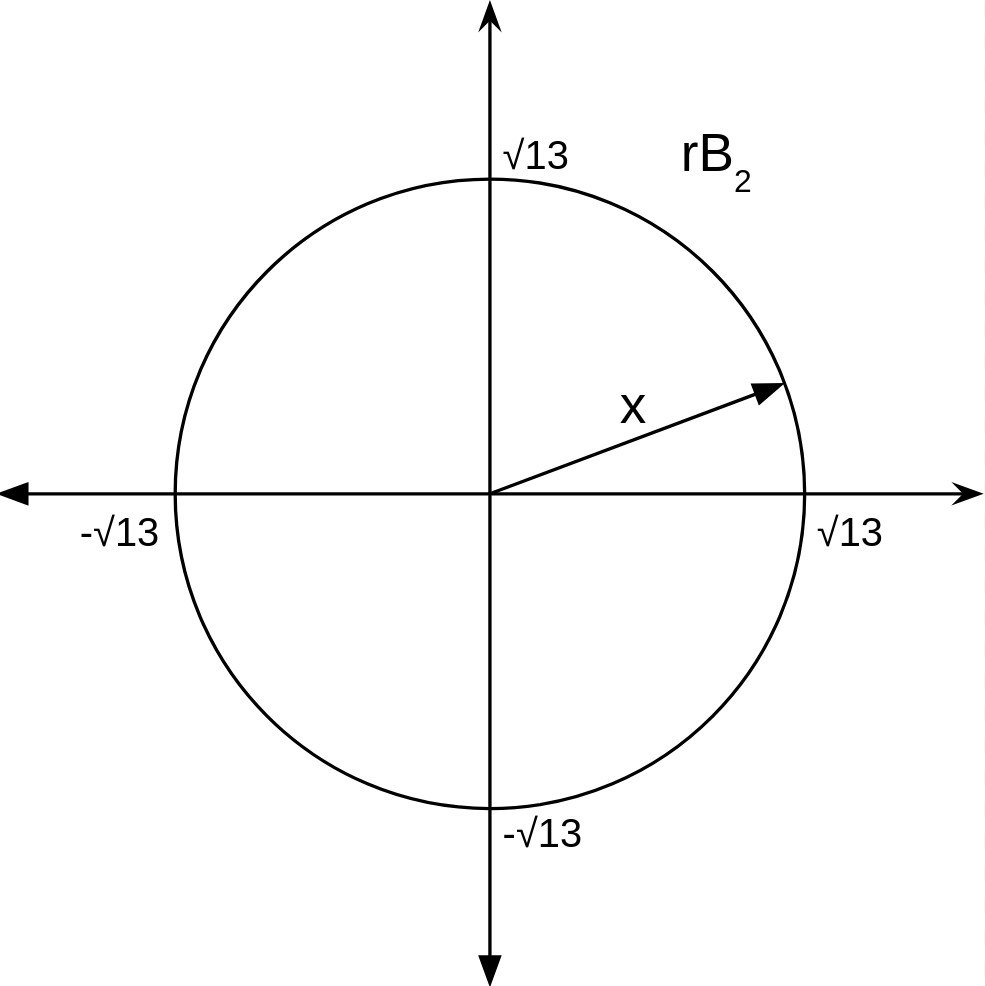
\includegraphics[scale=0.25]{l2.png}
\end{figure}

\begin{framed}
\[\|x\|_\infty=\text{max}(3,2)=3\]
\end{framed}
\begin{figure}[h]
    \caption{Plot of $x$ and $rB_\infty$}
    \centering
    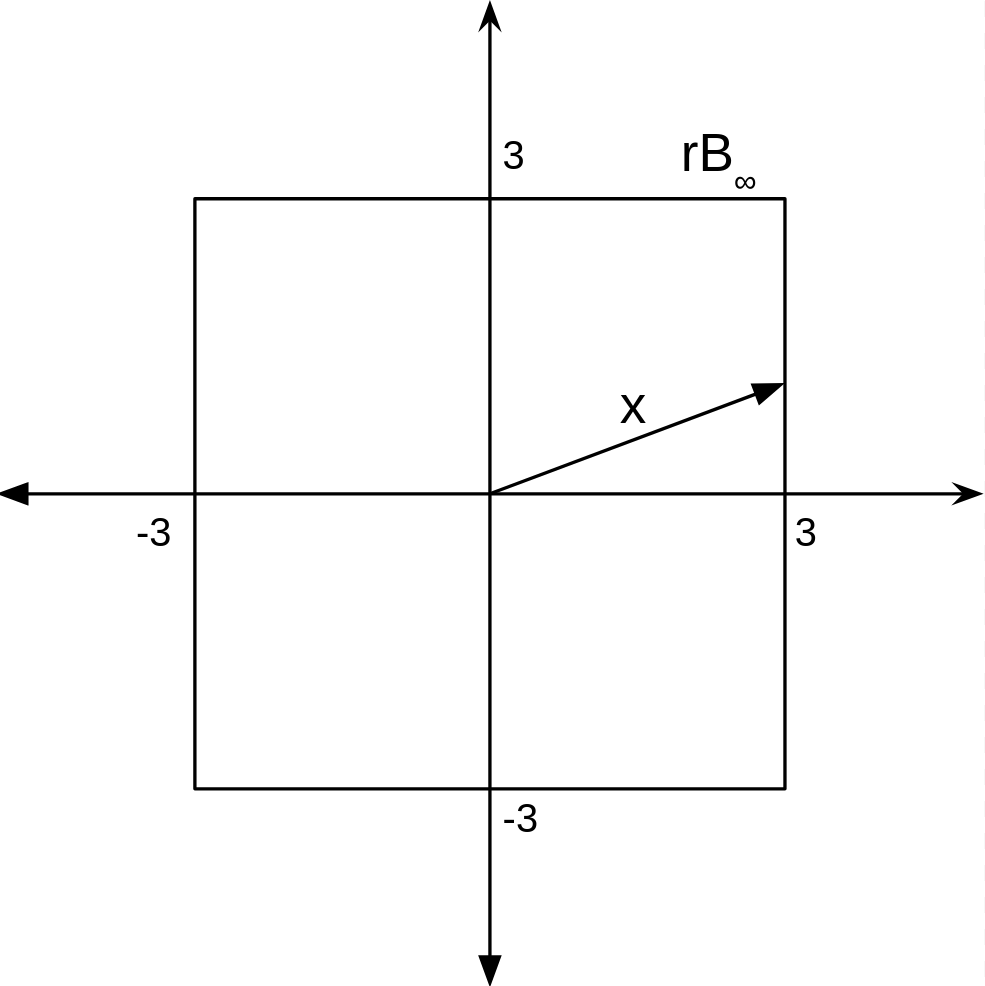
\includegraphics[scale=0.25]{linf.png}
\end{figure}

\newpage

b) Consider the following shapes and determine which $||\;\;||_{B_j}$ is a valid norm.

\begin{figure}[h]
    \caption{Plots of $B_p$}
    \centering
    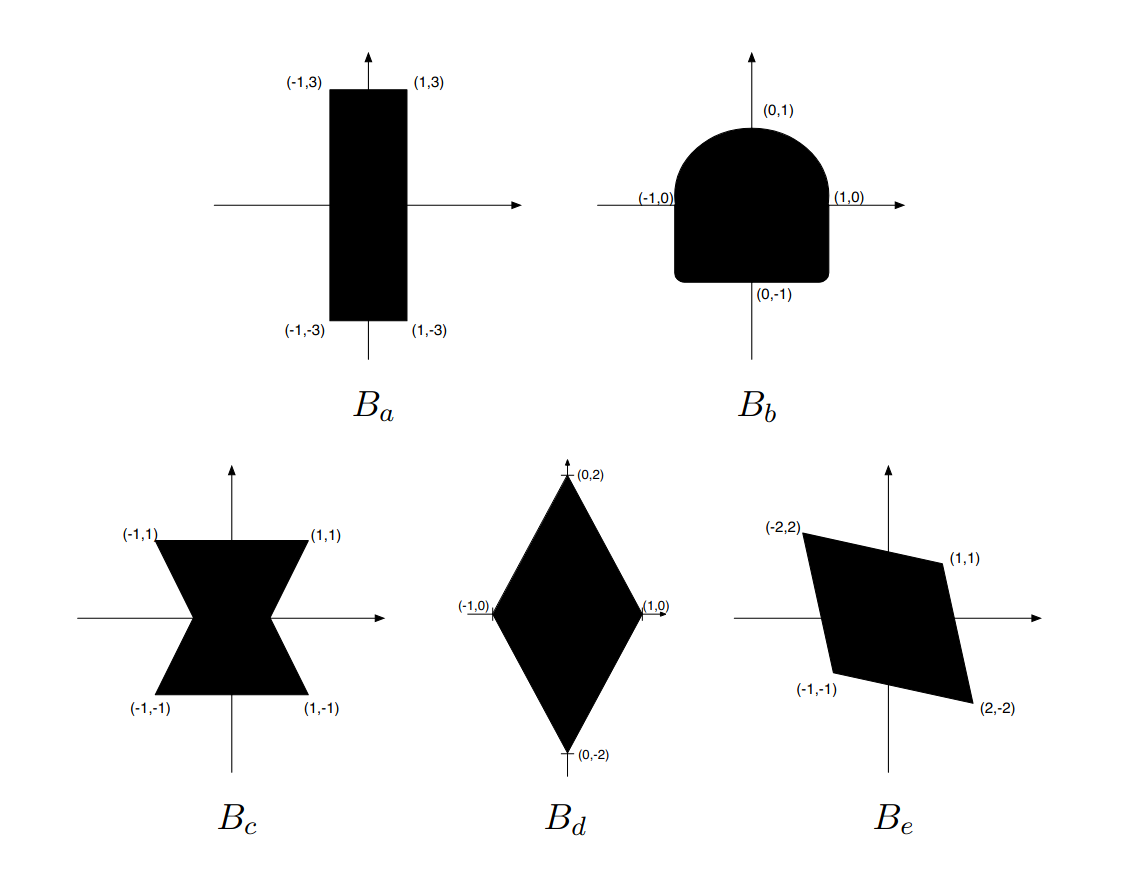
\includegraphics[scale=0.25]{normshapes.png}
\end{figure}

$B_a$ is a valid norm.

$B_b$ is not a valid norm. It violates the homogeneity property of a valid norm.

\[x=\begin{bmatrix}1\\1\end{bmatrix},\quad a=-1\]
\[\|ax\|\neq|a|\;\|x\|\]
\[\|-x|\|\neq\|x\|\]
\[\frac{1}{\sqrt{2}}\neq1\quad\text{The shape is not symetric}\]

$B_c$ is not a valid norm: It violates the triangle inequality.

\[x=\begin{bmatrix}1\\1\end{bmatrix},\quad y=\begin{bmatrix}1\\-1\end{bmatrix}\]
\[\|x\|=\|y\|=1\]
\[\|x+y\|>2\]
$x+y=\begin{bmatrix}2\\0\end{bmatrix}$ and due to $B_c$'s concavity, $B_c < 1$ where $y=0$ and $x>0$,
so $B_c$ must be scaled by more than 2 to so that $x\in rB_p$.
\[\|x\|+\|y\|<\|x+y\|\]

$B_d$ is a valid norm.

$B_e$ is a valid norm:
 
\begin{framed}
$j=a,d,e$ are valid norms. $j=b$ is not a valid norm because it violates the homogeneity property. $j=c$
is not a valid norm because it violates the triangle inequality.
\end{framed}

\end{enumerate}

I'm sorry, but this took way too much effort in LaTeX. I'll still use it when convenient, but I can't do
this for every assignment. Apologies.

\end{document}
